% !TeX root = tcolorbox.tex
% include file of tcolorbox.tex (manual of the LaTeX package tcolorbox)
\clearpage
\section{创建文本框的宏}%
\tcbset{external/prefix=external/coremacros_}%
%\subsection{Using \texttt{tcolorbox} and \texttt{\texorpdfstring{\char`\\}{\textbackslash}tcbox}}\label{subsec:macros_using}
\subsection{使用 \texttt{tcolorbox} 与 \texttt{\textbackslash tcbox}}\label{subsec:macros_using}
\begin{docEnvironment}{tcolorbox}{\oarg{options}}
  这是用于创建带圆角、可强调的彩色文本框的主要环境，
  该文本框还可选择分为两部分。文本框的外观由众多选项控制。
  在最简单的情形下，如下源代码

\begin{dispListing}
\begin{tcolorbox}
This is a \textbf{tcolorbox}.
\end{tcolorbox}
\end{dispListing}

会生成如下编译后的文本框：
\begin{tcolorbox}
这是一个 \textbf{tcolorbox}。
\end{tcolorbox}

框内文本可通过命令 \refCom{tcblower} 分为上部和下部。
在视觉上，两部分由一条分隔线隔开。例如：

\begin{dispListing}
\begin{tcolorbox}
This is another \textbf{tcolorbox}.
\tcblower
Here, you see the lower part of the box.
\end{tcolorbox}
\end{dispListing}

该代码生成如下文本框：
\begin{tcolorbox}
这是另一个 \textbf{tcolorbox}。
\tcblower
这里你看到的是文本框的下部。
\end{tcolorbox}

\meta{选项}用于控制文本框的外观与若干功能，完整列表参见 \zvref{sec:optkeys}。
这里给出一个简单示例：

\begin{dispExample}
\begin{tcolorbox}[colback=red!5!white,colframe=red!75!black,title=My nice heading]
This is another \textbf{tcolorbox}.
\tcblower
Here, you see the lower part of the box.
\end{tcolorbox}
\end{dispExample}
\end{docEnvironment}


\begin{docCommand}{tcblower}{}
  在 \refEnv{tcolorbox} 内部使用，用于将上部与可选的下部分隔开。
  上部和下部被视为相互独立的功能单元。
  若你只想画一条分隔线，请参见 \refCom{tcbline}。
\end{docCommand}


\clearpage
\begin{docCommand}{tcbset}{\marg{options}}
  在当前 \TeX\ 分组内，为其后的每个 \refEnv{tcolorbox} 设置选项。
  默认情况下，这不适用于嵌套文本框，参见 \zvref{subsec:everybox}。\par
  例如，可用以下方式为整个文档定义文本框的颜色：
\begin{dispListing}
\tcbset{colback=red!5!white,colframe=red!75!black}
\end{dispListing}
\end{docCommand}


\begin{docCommand}{tcbsetforeverylayer}{\marg{options}}
  在当前 \TeX\ 分组内，为其后的每个 \refEnv{tcolorbox} 设置选项。
  与 \refCom{tcbset} 不同，它同样作用于嵌套文本框，
  参见 \zvref{subsec:everybox}。
  从技术上讲，\meta{选项}会被追加到由 \refKey{/tcb/reset} 应用的
  每个 |tcolorbox| 的默认值之后。\par
  如果你不能完全确定是否希望这些 \meta{选项}也作用于
  框中框（乃至框中框中框……）中的文本框，则不应使用此宏。
\begin{dispExample}
\tcbset{colback=green!10!white}
\tcbsetforeverylayer{colframe=red!75!black}

\begin{tcolorbox}[title=All options for this box]
  This is a tcolorbox.\par\medskip
  \begin{tcolorbox}[title=Nested box]
    Note that this nested box has a red frame but no green background.
  \end{tcolorbox}
\end{tcolorbox}
\bigskip

\begin{tcolorbox}[reset]
  Options given with |\tcbsetforeverylayer| survive a |reset|.
\end{tcolorbox}
\end{dispExample}
\end{docCommand}


\clearpage
\begin{docCommand}{tcbox}{\oarg{options}\marg{box content}}
  创建一个彩色文本框，其宽度恰好贴合所给 \meta{框内容} 的宽度。
  原则上，\refEnv{tcolorbox} 的大多数 \meta{选项}都可用于 |\tcbox|，
  但有若干限制。|\tcbox| 不能有下部，也不能断开。

\begin{dispExample}
\tcbset{colframe=blue!50!black,colback=white,colupper=red!50!black,
        fonttitle=\bfseries,nobeforeafter,center title}

Text \tcbox[tcbox raise base]{Hello World}\hfill
%
\tcbox[left=0mm,right=0mm,top=0mm,bottom=0mm,boxsep=0mm,
  toptitle=0.5mm,bottomtitle=0.5mm,title=My table]{%
  \arrayrulecolor{blue!50!black}\renewcommand{\arraystretch}{1.2}%
  \begin{tabular}{r|c|l}
  One   & Two    & Three \\\hline\hline
  Men   & Mice   & Lions \\\hline
  Upper & Middle & Lower
  \end{tabular}}\hfill
%
\tcbox[colback=blue!85!black,
  left=0mm,right=0mm,top=0mm,bottom=0mm,boxsep=1mm,arc=0mm,boxrule=0.5pt,
  title=My picture]{%
  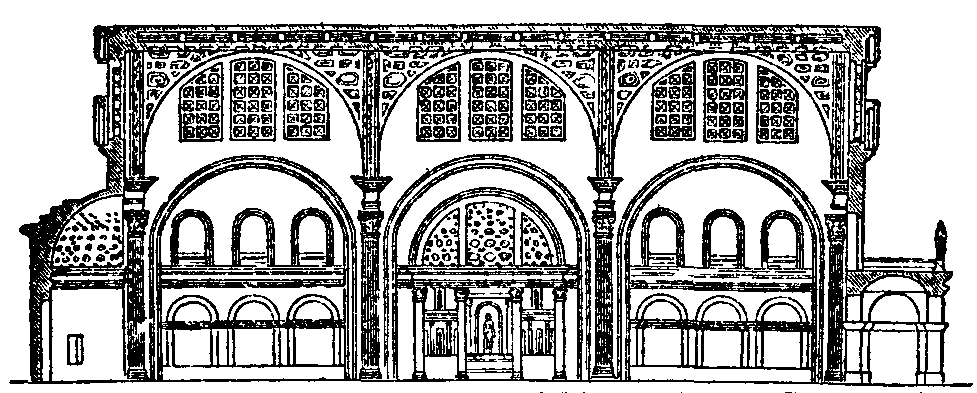
\includegraphics[width=5cm]{Basilica_5.png}}
\end{dispExample}

\begin{dispExample}
\tcbset{colframe=blue!50!black,colback=white,colupper=red!50!black,
        fonttitle=\bfseries,center title}

% Fixed width box
\begin{tcolorbox}Hello\\World!\end{tcolorbox}

% Fitted width box (like hbox or makebox)
\tcbox{Hello\\World!}

% Fitted width box (using a TikZ node)
\tcbox[tikznode]{Hello\\World!}
\end{dispExample}

\end{docCommand}


\clearpage

\begin{docCommand}{tcboxverb}{\oarg{options}\marg{verbatim box content}}
  在 \refCom{tcbox} 基础上创建一个彩色文本框，其宽度恰好贴合所给
  \meta{逐字框内容} 的宽度。底层的 \refCom{tcbox} 采用
  \refKey{/tcb/verbatim} 样式并叠加所给 \meta{选项}。
  与 \refCom{tcbox} 的区别在于，\meta{逐字框内容}会被逐字（\textit{verbatim}）解释。
  因此 |\tcboxverb| 的行为类似于 |\verb|。

\begin{dispExample}
\tcboxverb{\LaTeX}, \tcboxverb[colback=blue!10!white,colupper=blue]{\LaTeX},
\tcboxverb[blank,fuzzy halo]{\LaTeX}, \tcboxverb[beamer]{\LaTeX},
\tcboxverb[enhanced,skin=enhancedmiddle jigsaw,colframe=red]{\LaTeX}.
\end{dispExample}
\end{docCommand}

\clearpage
\subsection{生成 \texttt{tcolorbox} 环境与命令}\label{subsec:macros_tcolorbox}

\begin{docCommand}{newtcolorbox}{\oarg{init options}\marg{name}\oarg{number}\oarg{default}\marg{options}}
  基于 \refEnv{tcolorbox} 创建一个名为 \meta{name} 的新环境。
  基本上，|\newtcolorbox| 的用法与 |\newenvironment| 相同。
  这意味着新环境 \meta{name} 可带 \meta{number} 个参数，
  其中 \meta{default} 是第一个可选参数的默认值。
  \meta{选项}会传递给底层的 |tcolorbox|。
  注意，\refKey{/tcb/savedelimiter} 会自动设为所给的 \meta{name}。
  \meta{初始化选项}可用于设置自动编号，参见 \zvref{sec:initkeys}。
\begin{dispExample*}{sbs,lefthand ratio=0.6}
\newtcolorbox{mybox}{colback=red!5!white,
  colframe=red!75!black}

\begin{mybox}
This is my own box.
\end{mybox}
\end{dispExample*}

\begin{dispExample*}{sbs,lefthand ratio=0.6}
\newtcolorbox{mybox}[1]{colback=red!5!white,
  colframe=red!75!black,fonttitle=\bfseries,
  title={#1}}

\begin{mybox}{Hello there}
This is my own box with a mandatory title.
\end{mybox}
\end{dispExample*}

\begin{dispExample*}{sbs,lefthand ratio=0.6}
\newtcolorbox{mybox}[2][]{colback=red!5!white,
  colframe=red!75!black,fonttitle=\bfseries,
  colbacktitle=red!85!black,enhanced,
attach boxed title to top center={yshift=-2mm},
  title={#2},#1}

\begin{mybox}[colback=yellow]{Hello there}
This is my own box with a mandatory title
and options.
\end{mybox}
\end{dispExample*}

\inputpreamblelisting{A}

\begin{dispExample*}{sbs,lefthand ratio=0.6}
\begin{pabox}[colback=yellow]{Hello there}
This is my own box with a mandatory
numbered title and options.
\end{pabox}
\end{dispExample*}
\end{docCommand}


\begin{docCommand}{renewtcolorbox}{\oarg{init options}\marg{name}\oarg{number}\oarg{default}\marg{options}}
  用法与 \refCom{newtcolorbox} 相同，但基于 |\renewenvironment| 而非 |\newenvironment|。
  用于重新定义一个已存在的环境。
\end{docCommand}


\clearpage

\begin{docCommand}{NewTColorBox}{\oarg{init options}\marg{name}\marg{specification}\marg{options}}
  基于 \refEnv{tcolorbox} 创建一个名为 \meta{name} 的新环境。\\
  基本上，\refCom{NewTColorBox} 的用法与 |\NewDocumentEnvironment| 相同。
  这意味着新环境 \meta{name} 按照所给的 \LaTeX3 参数 \meta{语法说明}构造，
  详见 \cite{latexproject:usrguide}。
  若名为 \meta{name} 的环境已定义，则会报错。
  \meta{选项}会传递给底层的 \refEnv{tcolorbox}。\\
  注意，\refKey{/tcb/savedelimiter} 会自动设为所给的 \meta{name}。\\
  \meta{初始化选项}可用于设置自动编号，参见 \zvref{sec:initkeys}。

\begin{dispExample}
% counter from previous example
\NewTColorBox[use counter from=pabox]{mybox}{ O{red} m d"" !O{} }
  {enhanced,colframe=#1!75!black,colback=#1!5!white,
   fonttitle=\bfseries,title={\thetcbcounter~#2},
   IfValueT={#3}{watermark text={#3}},#4}

\begin{mybox}{My title}
This is a tcolorbox.
\end{mybox}

\begin{mybox}[blue]{My title}
This is a tcolorbox.
\end{mybox}

\begin{mybox}[green]{My title}"My Watermark"
This is a tcolorbox.
\end{mybox}

\begin{mybox}[yellow]{My title}[colbacktitle=yellow!50!white,coltitle=black]
This is a tcolorbox.
\end{mybox}

\begin{mybox}[purple]{My title}"All together"[coltitle=yellow]
This is a tcolorbox.
\end{mybox}
\end{dispExample}
\end{docCommand}

\clearpage
\begin{docCommand}{RenewTColorBox}{\oarg{init options}\marg{name}\marg{specification}\marg{options}}
  用法与 \refCom{NewTColorBox} 相同，但基于 |\RenewDocumentEnvironment| 而非 |\NewDocumentEnvironment|。
  用于重新定义一个已存在的环境。
\end{docCommand}

\begin{docCommand}{ProvideTColorBox}{\oarg{init options}\marg{name}\marg{specification}\marg{options}}
  用法与 \refCom{NewTColorBox} 相同，但基于 |\ProvideDocumentEnvironment| 而非 |\NewDocumentEnvironment|。
  仅当环境 \meta{name} 尚未定义时才创建它。
\end{docCommand}

\begin{docCommand}{DeclareTColorBox}{\oarg{init options}\marg{name}\marg{specification}\marg{options}}
  用法与 \refCom{NewTColorBox} 相同，但基于 |\DeclareDocumentEnvironment| 而非 |\NewDocumentEnvironment|。
  无论是否已存在同名环境，总是创建新环境。
\end{docCommand}


\clearpage

\begin{docCommand}{NewTotalTColorBox}{\oarg{init options}\brackets{\texttt{\textbackslash}\meta{name}}\marg{specification}\marg{options}\marg{content}}
  基于 \refEnv{tcolorbox} 创建一个新命令 \texttt{\textbackslash}\meta{name}。
  与 \refCom{NewTColorBox} 不同，这里还指定了 |tcolorbox| 的 \meta{内容}。\\
  基本上，\refCom{NewTotalTColorBox} 的用法与 |\NewDocumentCommand| 相同。
  这意味着新命令 \texttt{\textbackslash}\meta{name} 按照所给的
  \LaTeX3 参数 \meta{语法说明}构造，详见 \cite{latexproject:usrguide}。
  若 \texttt{\textbackslash}\meta{name} 已定义，则会报错。
  \meta{选项}会传递给底层的 \refEnv{tcolorbox}，并用所指定的 \meta{内容}填充。\\
  注意，\refKey{/tcb/savedelimiter} 会自动设为所给的 \meta{name}。
  另请注意，\refKey{/tcb/saveto}、\refKey{/tcb/savelowerto} 与
  \refKey{/tcb/redirectlowerto} 不能与 \refCom{NewTotalTColorBox} 及其同类命令一起使用。\\
  \meta{初始化选项}可用于设置自动编号，参见 \zvref{sec:initkeys}。

\begin{dispExample}
\NewTotalTColorBox{\diabox}{ O{} v  m }
  { bicolor,nobeforeafter,equal height group=diabox,width=5.7cm,
    fonttitle=\bfseries\ttfamily,adjusted title={#2},center title,
    colframe=blue!20!black,leftupper=0mm,rightupper=0mm,colback=black!75!white,#1}
  { \tikz\path[fill zoom image={#2}] (0,0) rectangle (\linewidth,4cm);%
    \tcblower#3}

\diabox{blueshade.png}{Created with |GIMP|.\\\url{http://www.gimp.org}}
\diabox{goldshade.png}{Created with |GIMP|.\\\url{http://www.gimp.org}}
\end{dispExample}
\end{docCommand}

\begin{docCommand}{RenewTotalTColorBox}{\oarg{init options}\brackets{\texttt{\textbackslash}\meta{name}}\marg{specification}\marg{options}\marg{content}}
  用法与 \refCom{NewTotalTColorBox} 相同，但基于 |\RenewDocumentCommand| 而非 |\NewDocumentCommand|。
  用于重新定义一个已存在的命令。
\end{docCommand}

\begin{docCommand}{ProvideTotalTColorBox}{\oarg{init options}\brackets{\texttt{\textbackslash}\meta{name}}\marg{specification}\marg{options}\marg{content}}
  用法与 \refCom{NewTotalTColorBox} 相同，但基于 |\ProvideDocumentCommand| 而非 |\NewDocumentCommand|。
  仅当命令 \texttt{\textbackslash}\meta{name} 尚未定义时才创建它。
\end{docCommand}

\begin{docCommand}{DeclareTotalTColorBox}{\oarg{init options}\brackets{\texttt{\textbackslash}\meta{name}}\marg{specification}\marg{options}\marg{content}}
  用法与 \refCom{NewTotalTColorBox} 相同，但基于 |\DeclareDocumentCommand| 而非 |\NewDocumentCommand|。
  无论是否已存在同名命令，总是创建新命令。
\end{docCommand}


\clearpage
\subsection{生成 \texttt{\textbackslash tcbox} 命令}\label{subsec:macros_tcbox}
\enlargethispage*{10mm}

\begin{docCommand}{newtcbox}{\oarg{init options}\brackets{\texttt{\textbackslash}\meta{name}}\oarg{number}\oarg{default}\marg{options}}
  基于 \refCom{tcbox} 创建一个新宏 \texttt{\textbackslash}\meta{name}。
  基本上，|\newtcbox| 的用法与 |\newcommand| 相同。
  新宏 \texttt{\textbackslash}\meta{name} 可带 \meta{number}$+1$ 个参数（最多 10 个），
  其中 \meta{default} 是第一个可选参数的默认值。
  除 \meta{number} 个参数外，\texttt{\textbackslash}\meta{name} 还自动带有一个
  末尾的（必填）参数，用于接收文本框内容。
  \meta{选项}会传递给底层的 |\tcbox|。
  \meta{初始化选项}可用于设置自动编号，参见 \zvref{sec:initkeys}。
\begin{dispExample*}{sbs,lefthand ratio=0.6}
\newtcbox{\mybox}{colback=red!5!white,
  colframe=red!75!black}

\mybox{This is my own box.}
\end{dispExample*}

\begin{dispExample*}{sbs,lefthand ratio=0.6}
\newtcbox{\mybox}[1]{colback=red!5!white,
  colframe=red!75!black,fonttitle=\bfseries,
  title={#1}}

\mybox{Hello there}{This is my own box.}
\end{dispExample*}

\begin{dispExample*}{sbs,lefthand ratio=0.6}
\newtcbox{\mybox}[2][]{colback=red!5!white,
  colframe=red!75!black,fonttitle=\bfseries,
  title={#2},#1}

\mybox[colback=yellow]{Hello there}%
  {This is my own box.}
\end{dispExample*}

\inputpreamblelisting{B}

\begin{dispExample*}{sbs,lefthand ratio=0.6}
\pbbox[colback=yellow]{Hello there}%
  {This is my own box.}
\end{dispExample*}

\begin{dispExample}
\newtcbox{\mybox}[1][red]{on line,
  arc=0pt,outer arc=0pt,colback=#1!10!white,colframe=#1!50!black,
  boxsep=0pt,left=1pt,right=1pt,top=2pt,bottom=2pt,
  boxrule=0pt,bottomrule=1pt,toprule=1pt}
\newtcbox{\xmybox}[1][red]{on line,
  arc=7pt,colback=#1!10!white,colframe=#1!50!black,
  before upper={\rule[-3pt]{0pt}{10pt}},boxrule=1pt,
  boxsep=0pt,left=6pt,right=6pt,top=2pt,bottom=2pt}

The \mybox[green]{quick} brown \mybox{fox} \mybox[blue]{jumps} over the
\mybox[green]{lazy} \mybox{dog}.\par
The \xmybox[green]{quick} brown \xmybox{fox} \xmybox[blue]{jumps} over the
\xmybox[green]{lazy} \xmybox{dog}.
\end{dispExample}
\end{docCommand}


\clearpage
\begin{docCommand}{renewtcbox}{\oarg{init options}\brackets{\texttt{\textbackslash}\rmfamily\meta{name}}\oarg{number}\oarg{default}\marg{options}}
  用法与 \refCom{newtcbox} 相同，但基于 |\renewcommand| 而非 |\newcommand|。
  用于重新定义一个已存在的宏。
\end{docCommand}


\begin{docCommand}{NewTCBox}{\oarg{init options}\brackets{\texttt{\textbackslash}\meta{name}}\marg{specification}\marg{options}}
  基于 \refCom{tcbox} 创建一个新命令 \texttt{\textbackslash}\meta{name}。
  基本上，\refCom{NewTCBox} 的用法与 |\NewDocumentCommand| 相同。
  这意味着新命令 \texttt{\textbackslash}\meta{name} 按照所给的
  \LaTeX3 参数 \meta{语法说明}构造，详见 \cite{latexproject:usrguide}。
  除参数 \meta{语法说明}外，\texttt{\textbackslash}\meta{name} 还自动带有一个
  末尾的（必填）参数，用于接收文本框内容。
  因此，\texttt{\textbackslash}\meta{name} 总共最多可带 10 个参数。
  若 \texttt{\textbackslash}\meta{name} 已定义，则会报错。
  \meta{选项}会传递给底层的 \refCom{tcbox}。\\
  注意，\refKey{/tcb/savedelimiter} 会自动设为所给的 \meta{name}。\\
  \meta{初始化选项}可用于设置自动编号，参见 \zvref{sec:initkeys}。

\begin{dispExample}
% counter from previous example
\NewTCBox[use counter from=pabox]{\mybox}{ s m s }
{ nobeforeafter,colback=red!5!white,colframe=red!75!black,
  title={#2 (Box \thetcbcounter)},fonttitle=\bfseries,
  IfBooleanT={#1}{enhanced,drop shadow},
  IfBooleanT={#3}{colbacktitle=red!50!white} }

\mybox{Bird}{This is my first box.}
  \hfill
\mybox*{Tree}{This is my second box.}
  \par\bigskip
\mybox{Bike}*{This is my third box.}
  \hfill
\mybox*{City}*{This is my fourth box.}
\end{dispExample}
\end{docCommand}


\begin{docCommand}{RenewTCBox}{\oarg{init options}\brackets{\texttt{\textbackslash}\meta{name}}\marg{specification}\marg{options}}
  用法与 \refCom{NewTCBox} 相同，但基于 |\RenewDocumentCommand| 而非 |\NewDocumentCommand|。
  用于重新定义一个已存在的命令。
\end{docCommand}

\begin{docCommand}{ProvideTCBox}{\oarg{init options}\brackets{\texttt{\textbackslash}\meta{name}}\marg{specification}\marg{options}}
  用法与 \refCom{NewTCBox} 相同，但基于 |\ProvideDocumentCommand| 而非 |\NewDocumentCommand|。
  仅当命令 \texttt{\textbackslash}\meta{name} 尚未定义时才创建它。
\end{docCommand}

\begin{docCommand}{DeclareTCBox}{\oarg{init options}\brackets{\texttt{\textbackslash}\meta{name}}\marg{specification}\marg{options}}
  用法与 \refCom{NewTCBox} 相同，但基于 |\DeclareDocumentCommand| 而非 |\NewDocumentCommand|。
  无论是否已存在同名命令，总是创建新命令。
\end{docCommand}


\clearpage

\begin{docCommand}{NewTotalTCBox}{\oarg{init options}\brackets{\texttt{\textbackslash}\meta{name}}\marg{specification}\marg{options}\marg{content}}
  基于 \refCom{tcbox} 创建一个新命令 \texttt{\textbackslash}\meta{name}。
  与 \refCom{NewTCBox} 不同，这里还指定了 |\tcbox| 的 \meta{内容}。\\
  基本上，\refCom{NewTotalTCBox} 的用法与 |\NewDocumentCommand| 相同。
  这意味着新命令 \texttt{\textbackslash}\meta{name} 按照所给的
  \LaTeX3 参数 \meta{语法说明}构造，详见 \cite{latexproject:usrguide}。
  若 \texttt{\textbackslash}\meta{name} 已定义，则会报错。
  \meta{选项}会传递给底层的 \refCom{tcbox}，并用所指定的 \meta{内容}填充。\\
  注意，\refKey{/tcb/savedelimiter} 会自动设为所给的 \meta{name}。\\
  \meta{初始化选项}可用于设置自动编号，参见 \zvref{sec:initkeys}。

\begin{dispExample}
\NewTotalTCBox{\myverb}{ O{red} v !O{} }
{ fontupper=\ttfamily,nobeforeafter,tcbox raise base,arc=0pt,outer arc=0pt,
  top=0pt,bottom=0pt,left=0mm,right=0mm,
  leftrule=0pt,rightrule=0pt,toprule=0.3mm,bottomrule=0.3mm,boxsep=0.5mm,
  colback=#1!10!white,colframe=#1!50!black,#3}{#2}

To set a word \textbf{bold} in \myverb{\LaTeX}, use
\myverb[green]{\textbf{bold}}. Alternatively, write
\myverb[yellow]{{\bfseries bold}}.
In \myverb[blue]{\LaTeX}[enhanced,fuzzy halo], other font settings are
done in the same way, e.\,g.\ \myverb{\textit}, \myverb{\itshape}\\
or \myverb[brown]{\texttt}, \myverb[brown]{\ttfamily}.
\end{dispExample}

下一个示例使用 \refPkg{listings} 宏包的 |\lstinline| 来排版逐字内容。

\begin{dispExample}
% \usepackage{listings} or \tcbuselibrary{listings}
\NewTotalTCBox{\commandbox}{ s v }
{verbatim,colupper=white,colback=black!75!white,colframe=black}
{\IfBooleanT{#1}{\textcolor{red}{\ttfamily\bfseries > }}%
  \lstinline[language=command.com,keywordstyle=\color{blue!35!white}\bfseries]^#2^}

\commandbox*{cd "My Documents"} changes to directory \commandbox{My Documents}.

\commandbox*{dir /A} lists the directory content.

\commandbox*{copy example.txt d:\target} copies \commandbox{example.txt} to
  \commandbox{d:\target}.
\end{dispExample}
\end{docCommand}

\clearpage

\begin{docCommand}{RenewTotalTCBox}{\oarg{init options}\brackets{\texttt{\textbackslash}\meta{name}}\marg{specification}\marg{options}\marg{content}}
  用法与 \refCom{NewTotalTCBox} 相同，但基于 |\RenewDocumentCommand| 而非 |\NewDocumentCommand|。
  用于重新定义一个已存在的命令。
\end{docCommand}

\begin{docCommand}{ProvideTotalTCBox}{\oarg{init options}\brackets{\texttt{\textbackslash}\meta{name}}\marg{specification}\marg{options}\marg{content}}
  用法与 \refCom{NewTotalTCBox} 相同，但基于 |\ProvideDocumentCommand| 而非 |\NewDocumentCommand|。
  仅当命令 \texttt{\textbackslash}\meta{name} 尚未定义时才创建它。
\end{docCommand}

\begin{docCommand}{DeclareTotalTCBox}{\oarg{init options}\brackets{\texttt{\textbackslash}\meta{name}}\marg{specification}\marg{options}\marg{content}}
  用法与 \refCom{NewTotalTCBox} 相同，但基于 |\DeclareDocumentCommand| 而非 |\NewDocumentCommand|。
  无论是否已存在同名命令，总是创建新命令。
\end{docCommand}



%\clearpage
\subsection{重定义其他环境（用 \texttt{tcolorbox} 包裹）}\label{subsec:macros_refine}

\begin{docCommand}[doc new=2014-10-20]{tcolorboxenvironment}{\marg{name}\marg{options}}
  重新定义已存在的环境 \meta{name}，使其被包裹在一个采用所给
  \meta{选项}的 |tcolorbox| 中。
\begin{dispExample*}{sbs,lefthand ratio=0.6}
% tcbuselibrary{skins}
\newenvironment{myitemize}{%
  \begin{itemize}}{\end{itemize}}

\tcolorboxenvironment{myitemize}{blanker,
  before skip=6pt,after skip=6pt,
  borderline west={3mm}{0pt}{red}}

Some text.
\begin{myitemize}
\item Alpha
\item Beta
\item Gamma
\end{myitemize}
More text.
\end{dispExample*}

\medskip
更多示例参见 \zvref{subsec:theorems_other}。
\end{docCommand}

